\documentclass{article}

\usepackage{graphicx}
\usepackage{subcaption}

\title{AIML426 Project 1 Report}
\date{}

\begin{document}
\maketitle
\section*{Part 1}
\subsection*{Individual Representation}
For this GA the chromosome is represented through a bit vector whose length is the number of possible items to choose from, each element represents a possible item to select for the knapsack. For decoding the chromosome into a solution, for each bit, 1 represents selecting the item while 0 represents not selecting the item.  \par
\noindent Since the order of the items picked up does not matter, the order of items in the chromosome can be the same as the order of items in the weight and values list. This means that the value and weight can be easily obtained by looking at the index of the chosen item in the chromosome in the values and weights lists. The crossover and mutation genetic operators can easily be applied to the chromosome and the solution can be decoded no matter how much the chromosome has changed. \par
\subsubsection*{Individual Generation}
\noindent At first for individual generation a random bit list of range of items length was generated. This worked for the first two datasets, but a problem that was encountered with the third dataset is that it has a large range of items to select, but has a small weight constraint. Thus the majority of individual generated violated the constraint by a lot and the initial population have 0 total fitness and never improve for a long time. \par
\noindent To avoid this the constraint was implemented into the individual generation for the initial population so that all the individuals satisfied the constraint. This was done by starting with a 0 chromosome and setting bits to 1 randomly in the chromosome until the weight constraint has been reached. This will still give a diverse range of individuals while setting the initial population fitness to above 0 and thus having a greater chance of improving the overall population fitness before convergence. \par
\subsection*{Fitness Function}
The fitness of the knapsack solutions is measured in the maximum value of items chosen while also satisfying the maximum weight constraint. The evaluate the maximum value of the knapsack solution, the sum of values of the items selected is calculated. To implement the constraint a penalty variable is introduced, the formula that is used to evaluate when to use the penalty variable for individual of $M$ bits is 
\begin{center} 
$max(0, \sum_{i=1}^{M}v_i - \alpha *max(0,\sum_{i=1}^{M}w_i)-max weight)$. 
\end{center}
So, when the total weight of the solution is greater than the maximum weight, the penalty is applied. A minimum fitness of 0 is set since negative fitness does not work with probabilities.
\subsection*{Genetic Operators}
\subsubsection*{Crossover}
One-point crossover was used for the crossover genetic operator, since the order of the items selected does not matter, no constraints need to be defined for the split position of the crossover. 
\subsubsection*{Mutation}
Local search mutation was used for the mutation genetic operator. Instead of randomly selecting a bit and flipping the value, the flip position with the largest increase in value is selected. This does increase the computation requirement since instead of O(1) complexity it is now O(M) complexity requiring to now iterate through each possible flip, but also increase chance of improving population each generation and reaching convergence early since mutation will be less likely to produce individuals with bad fitness. 
\subsection*{GA Parameter Values}
%Generation Number and Population Size
\subsubsection*{Number of Generations and Population Size}
To achieve close to the optimal value, different population sizes and generation numbers was tuned for each dataset. For the first and second dataset, population size of 50 and generation number of 100 was set since the dataset is small, thus reaching the optimal value can be quicker. For the third dataset, because of the strict constraint, 100 was set for the population size since there are less individuals that will satisfy the constraint of this dataset. This does mean that running the GA for this dataset is very time consuming so the population size did not increase beyond 100.
%Generations until convergence
\subsubsection*{Iterations Until Convergence}
This was set to 5 so that convergence only occurs when it is obvious that the fitness, measured as the average of the top 5 best individuals, no longer changes each generation. Thus saving computation time with the GA avoiding a large number of iterations with no effect. If set too large, the computation time saved becomes small.
%Selection used
\subsubsection*{Selection Scheme Used}
A fitness-proportional/roulette wheel selection scheme is used for this problem. When implementing the roulette wheel selection, the probability: $\frac{fitness(i)}{pop\_fitness}$ is calculated. A higher probability means a higher chance of being selected either for elitism or for parents. This was chosen since a roulette wheel selection is simple to implement and it encourages selecting high fitness solutions through having a larger probability of being chosen. This is also where the maximum weight constraint is implemented through. 
%Alpha value
\subsubsection*{Alpha/Penalty Coefficient}
The penalty coefficient/alpha variable needs to be tuned to the dataset so it is strong enough to generally ignore solutions that violate constraint when selecting individuals, but small enough to still acknowledge solutions that only slightly violate constraint but have very good value sums. \par
\noindent For the first dataset, an alpha value of 2 was selected since the was a small range of items to select from. \par
\noindent For the second dataset, there was a greater range of items to select from so the alpha value was higher to 3. \par
\noindent For the third dataset, while there was a much greater range of items to select and the weight constraint was very small. Thus the alpha value was set very high to make sure that the best individual does not violate the constraint. \par
%Crossover, Mutation, Elitism rates
\subsubsection*{Crossover, Mutation and Elitism Rates}
For both the first and second dataset, the parameter rates used are: 
\begin{center}
\begin{tabular}{|c|c|}
	\hline
	Elitism Rate: & 0.03 \\
	\hline
	Crossover Rate: & 1.0 \\
	\hline
	Mutation Rate: & 0.3 \\
	\hline
\end{tabular}
\end{center}
For the third dataset, a much higher elitism rate was used to encourage more fit individuals for the next generation since fit individuals means that they do not violate the constraint which is difficult to achieve. The parameter rates used are:
\begin{center}
\begin{tabular}{|c|c|}
	\hline
	Elitism Rate: & 0.1 \\
	\hline
	Crossover Rate: & 1.0 \\
	\hline
	Mutation Rate:	& 0.3 \\
	\hline
\end{tabular}
\end{center}
\subsection*{Results}
%show tables here
\begin{figure}[h]
	\centering
	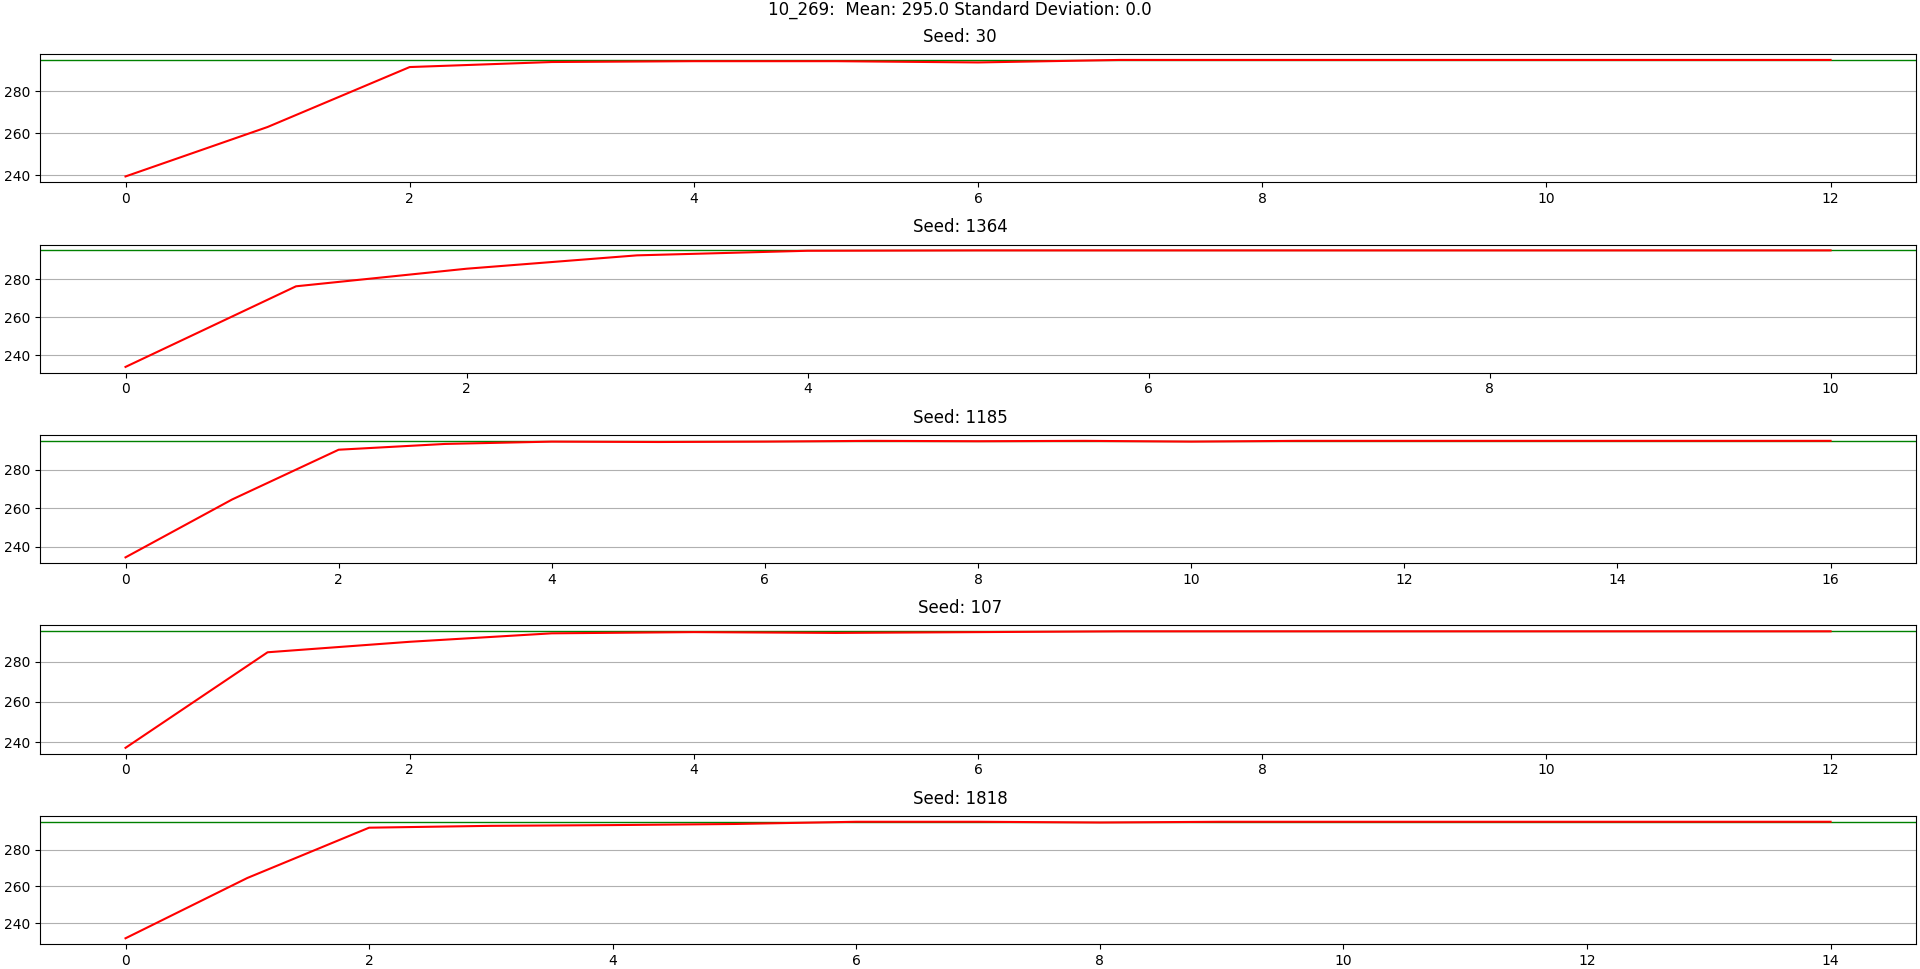
\includegraphics[width=\linewidth]{10_269.png}
	\caption{Convergence curves for dataset 10\_269. Original png image provided as well}
\end{figure}
\begin{figure}[h]
	\centering
	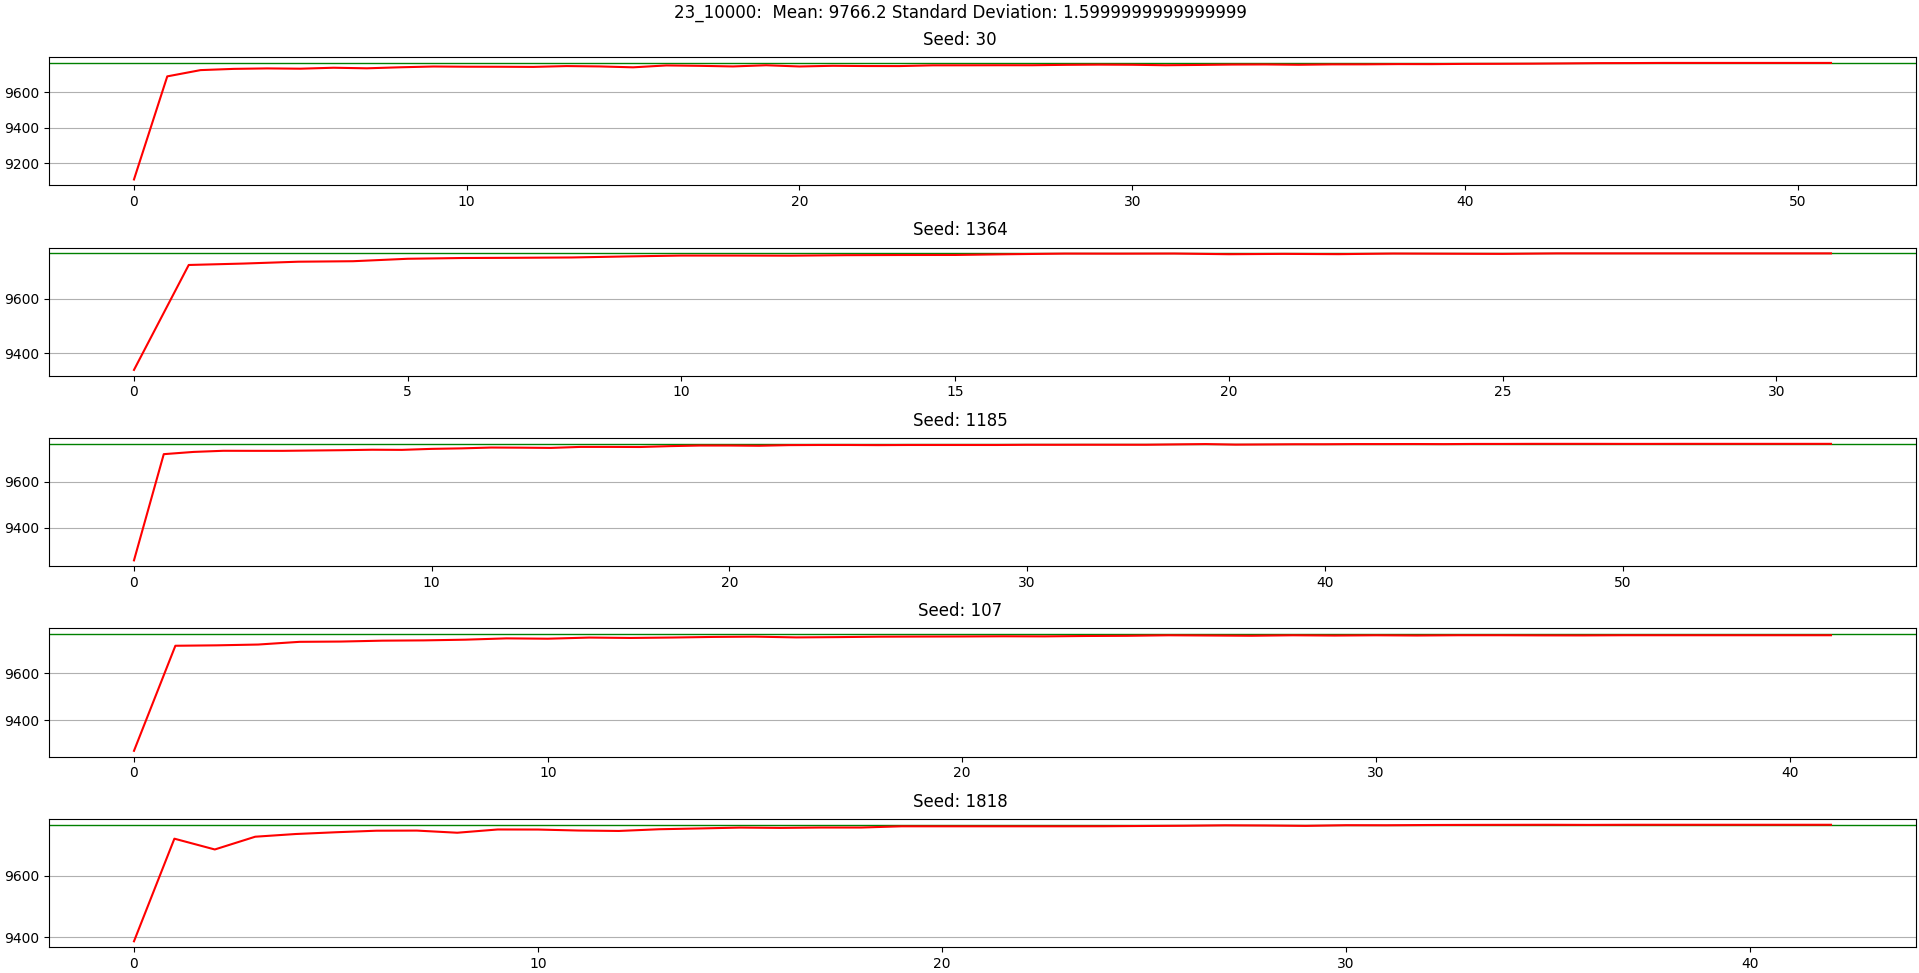
\includegraphics[width=\linewidth]{23_10000.png}
	\caption{Convergence curves for dataset 23\_10000. Original png image provided as well}
\end{figure}
\begin{figure}[h]
	\centering
	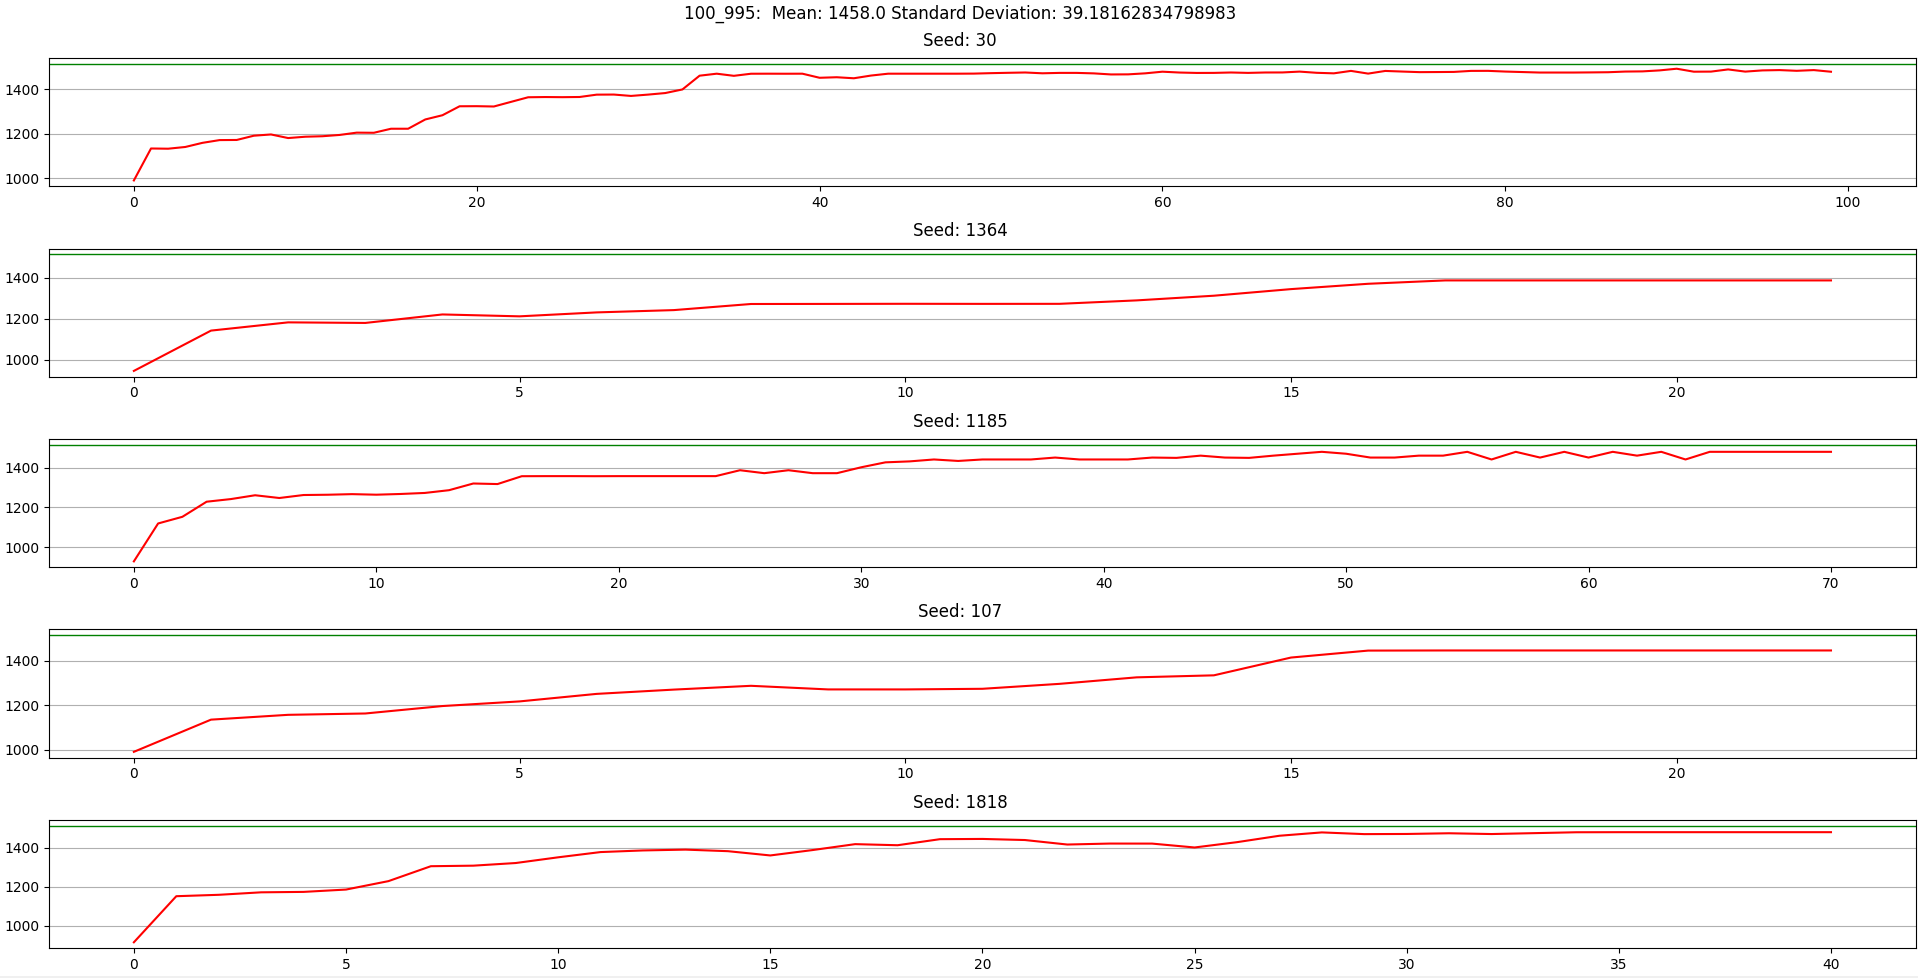
\includegraphics[width=\linewidth]{100_995.png}
	\caption{Convergence curves for dataset 100\_995. Original png image provided as well}
\end{figure}
\clearpage
%show best instance for the 5 seeds and datasets here
\begin{center}
\begin{tabular}{|c|c|}
	\hline
	Seed: & Best Individual Fitness: \\
	\hline
	\multicolumn{2}{|c|}{10\_269} \\
	\hline
	30 & 295	\\
	1364 & 295 \\
	1185 & 295 \\
	107 & 295 \\
	1181 & 295 \\
	\hline
	\multicolumn{2}{|c|}{23\_10000} \\
	\hline
	30	& 9767 \\
	1364 & 9767 \\
	1185 & 9767 \\
	107 & 9763 \\
	1181 & 9767 \\
	\hline
	\multicolumn{2}{|c|}{100\_995} \\
	\hline
	30	& 1481 \\
	1364 & 1479 \\
	1185 & 1324 \\
	107 & 1501 \\
	1181 & 1481 \\
	\hline
\end{tabular}
\end{center}
\subsubsection*{Discussion}
For 10\_269, this dataset converged to the optimal solution in < 20 generations for all seeds. That means the mean fitness is the same value as the optimal fitness with no deviation. The small range of items to pick from means that exploring all solutions is possible to achieve with GA. This showcases that with the population structure of GA, exploring a large range of solutions can be done within a few generations. \par
\noindent For 23\_10000 more generations were needed to reach the optimal solution. Four of the seeds achieved the optimal solution, but seed 107 was slightly under the optimal fitness. Creating a mean that is slightly less than the optimal fitness with small deviation. There is a logarithmic relation between the average best fitness of the generation with the number of generations showcasing that this dataset took a while to reach convergence despite being close to the optimal fitness. This could be circumvented by decreasing the mutation rate to prevent minor fitness changes in each generation that stopped convergence. \par
\noindent For 100\_995 none of the seeds reached the optimal solution of 1514 though four of the five seeds were close to the optimal solution. With the mean fitness being noticeably lower than the optimal fitness and with a large standard deviation, this showcases that the seed value has a bigger effect on the final solution compared to the other datasets. Since the weight constraint for this dataset was very small and there are a large range of items to select from, most of all the possible instances violate the constraint. Trying to find the few instances that satisfy the constraint while still trying to achieve a high value sum required finetuning of the parameters until a decent result was produced. Since all the seeds converged before reaching the maximum number of iterations, this showcases a higher rate of mutation was needed, but increasing the mutation rate also increases the likelihood of violating the constraint. The output could be improved with a higher population size, but more computation time would be needed. Several instances of the GA could be run with different seeds with the final output being the best output out of all the individual GA’s best output since different seed values produce variety while also satisfying the constraint. \par
\subsubsection*{Conclusion}
GA is a useful technique for finding optimal or near optimal solutions with it succeeding to finding optimal solutions for small datasets within a reasonable timeframe. The parameters used for the datasets could be worked on more to increase accuracy and performance of the GA to achieve a balance of searching through a large range of solutions without getting stuck in a local optima while still approaching the global optima over time. \par
\noindent GA does struggle with constraints, especially very strict constraints which most solutions violate. Since GAs can easily generate solutions that violate the constraint through reproduction. While implementing the penalty coefficient into the fitness evaluation can help define the constraint into the population, it needs to be balanced to encourage variety and sometimes still struggles to get solutions that are close to the optimal value while not violating the constraint. \par
\section*{Part 2}

\end{document}